\documentclass[12pt, letterpaper]{article}
\usepackage[utf8]{inputenc}
\usepackage{graphicx}
\graphicspath{ {./images/} }

\title{My Math Notes}
\author{John Lockwood \thanks{Special thanks to my lovely wife}}
\date{June 2022}

\newcommand\T{\rule{0pt}{8mm}}       % Top strut

\begin{document}

\maketitle

\section{Introduction}

What I want to be able to do is to keep important math notes handy.

\section{Unit Circle}
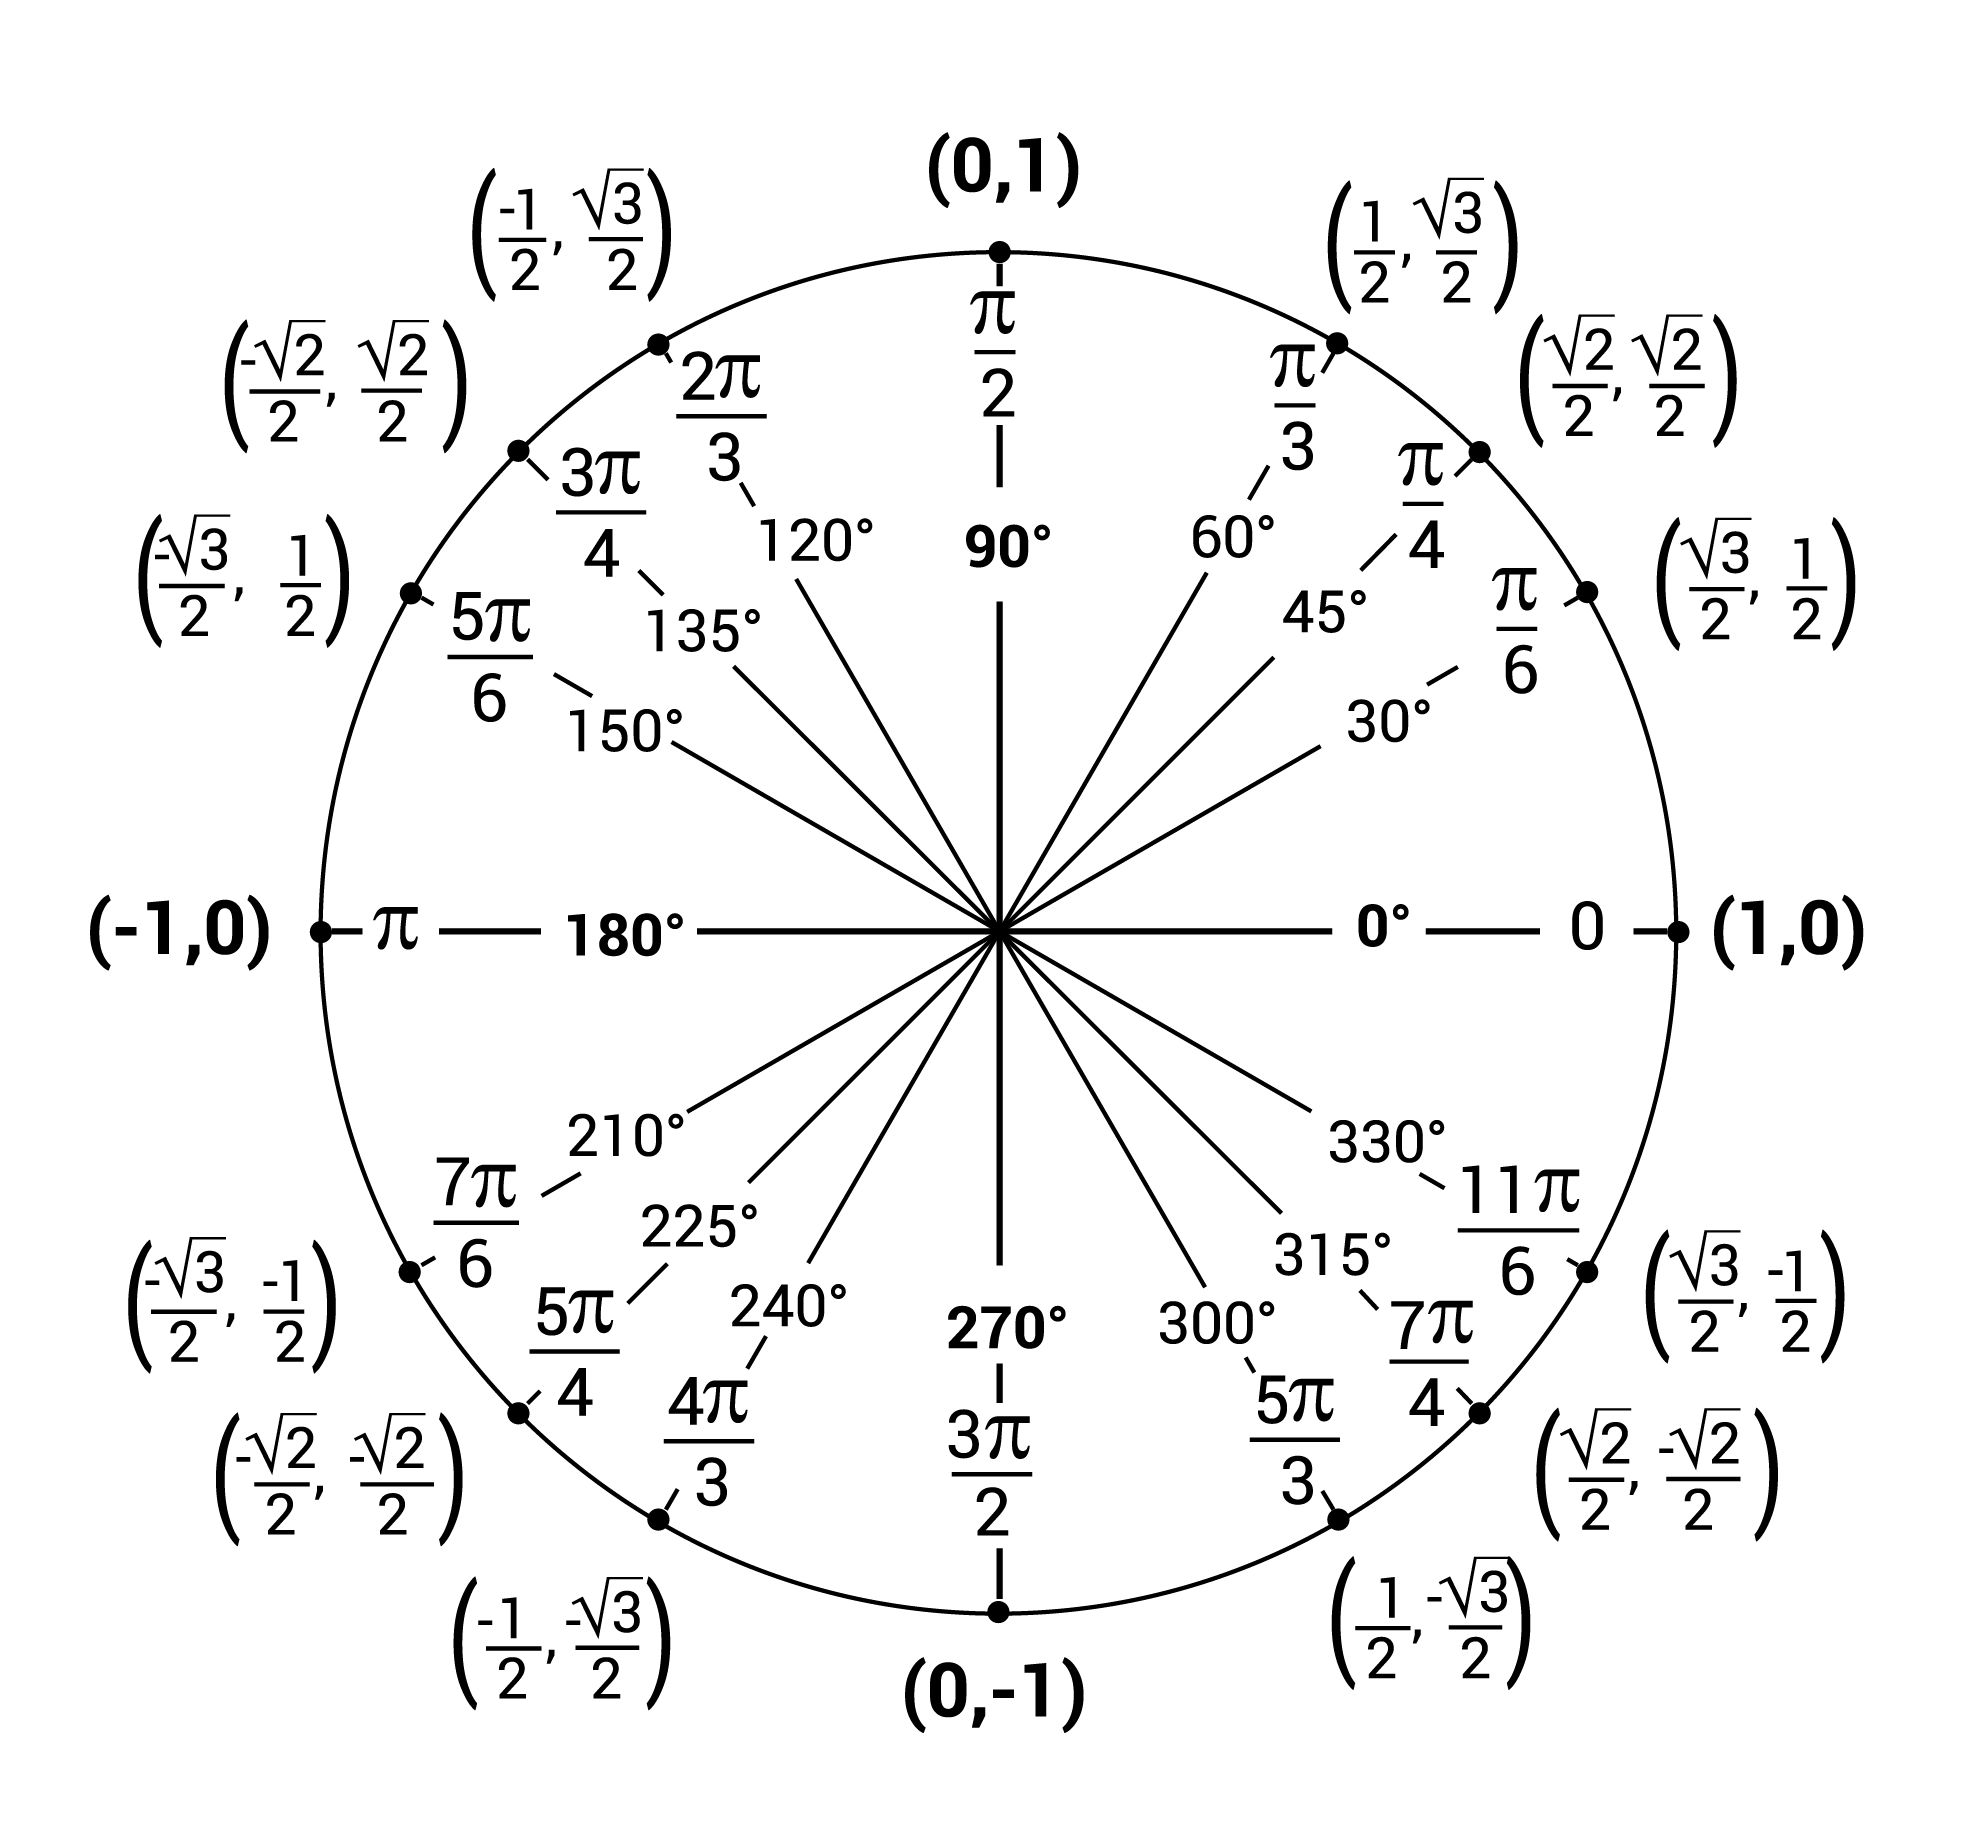
\includegraphics[width=6cm, height=6cm]{unit-circle.png}

\subsection{Some Baloney}

Some of the \textbf{best ideas} should show up in \underline{\textit{this document}}! 

\section{Trigonometric Identities}

\begin{center}
    \begin{tabular}{  p{5cm}  p{5cm} }
        $\csc x = \frac{1}{\sin x }$ & 
        $\sec x = \frac{1}{\cos x }$ \T \\
        
        $\cot x = \frac{1}{\tan x }$ & 
        $\tan x = \frac{sin x}{\cos x }$ \T \\
        $\cot x = \frac{cos x}{\sin x }$ & 
        $\sin^2 x + cos^2 = 1$ \T \\

\end{tabular}
\end{center}
\vspace{1cm}

\section{Parens}
$(\frac{f(x)}{g(x)})$
\end{document}
